% Summary index document for the analysis chapter
\chapter{Analyse}
\label{chap:Analyse}

\todo{Intro}
\todo{JAN: Kapitel überarbeiten, Analyse des Problems am Anfang.}

\section{Einführung}
Gemäss der Aufgabenstellung dieser \work{} ist die Programmiersprache für das \tool{} frei wählbar mit der einzigen Voraussetzung, dass man eine \acs{PCAP}-Library einbinden kann. In der Inception-Phase des Projekts ging es daher darum, eine geeignete Sprache und Bibliothek zu wählen.

\section{JNetPcap}
\label{sec:JNetPcap}

todo Jan

\section{Golang und goPacket}
\label{sec:Golang und goPacket}

\subsection{Golang}
Golang, auch Go genannt, ist eine eher junge Programmiersprache seit 2007 von Google Inc. entwickelt wurde. Golang hat einen C-ähnlichen Syntax, bietet aber viele Eigenschaften von modernen Programmiersprachen wie zum Beispiel Garbage Collection, Type-Safety, Dynamic-Typing, Closures und eine grosse Standard-Library.
Im Oktober 2009 wurde die Golang der Öffentlichkeit als Open Source zur Verfügung gestellt.

\subsection{Evaluation}
Unseren ersten Kontakt mit Golang haben wir durch GoProbe von Open Systems gewonnen.
GoProbe erlaubt leichtgewichtiges aggregieren von Paketen und deren effiziente Speicherung. Eine Abfrage der gespeicherten Paketen ist via Querying Flows möglich.


\section{Performance Vergleich}
\label{sec:Performance Vergleich}

\subsection{Testaufbau}
2 Desktop-Rechner der HSR sind via Gigabit-Lan miteinander verbunden. Auf den Rechnern läuft Ubuntu 14.04 x64 sowie jPerf und die jeweils getestete Software.

%todo Grafik mit MS Visio die unser Testaufbau darstellt.

\subsection{Testdurchführung}
Auf einem der beiden Rechnern läuft jeweils jPerf im Server-Modus sowie die getestete Software. Auf dem anderen Computer läuft jPerf im Client-Modus.
Via. jPerf wird nun soviel Traffic erzeugt um die 1Gbit/s-Leitung möglichst stark auszulasten, d.h. durchschnittlich 900mbit/s. Die getestete Software zeichnet dabei die ganzen Pakete auf und sollte dabei 300mbit/s an Traffic ertragen können. 300mbit/s sind gem. Open Systems AG die Lastspitzen mit denen etwa zu rechnen sind.

\subsection{Ergebnisse}
Java und Golang sind von den Ergebnissen her recht ähnlich. Beide haben die Anforderung von 300mbit/s erfolgreich erfüllt. Golang ist mit den Durchschnittlich 17\% CPU Auslastung etwas performanter als Java. Die 31\% CPU Lastspitze bei Java gibt es jeweils nur wenn das Programm zum ersten Mal gestartet wird und kommt daher dass dann die ganze \acs{JVM} zuerst hochgefahren werden muss.
Beim Memory siehts bei goProbe klar besser aus weil es den ganzen \acs{JVM} Overhead nicht hat.

\begin{table}[h]
\begin{tabular}{|l|l|l|l|}
\hline
\rowcolor[HTML]{C0C0C0} 
\textbf{Software} & \textbf{CPU Spitze} & \textbf{CPU Ø} & \textbf{Memory Ø} \\ \hline
JNetPcap auf Java & 31\%                & 20\%           & tbd               \\ \hline
goProbe auf Go    & 18\%                & 17\%           & tbd               \\ \hline
\end{tabular}
\end{table}

\section{Entscheidung}
Open Systems AG würde es bevorzugen, wenn Go statt Java verwendet wird. Die Ergebnisse des Performance-Tests sprechen ebenfalls für Go. Und wir haben durchaus auch das Interesse  eine neue Programmiersprache zu lernen.
In Anbetracht dessen haben wir uns entschieden, das \tool{} mit Go zu entwickeln.

\section{ESP Aufbau}
\label{sec:ESP Aufbau}

\noindent Encapsulating Security Payload (ESP) wird bei \ac{IPsec} (VPN) eingesetzt. Es gewährleistet die Vertraulichkeit und Integrität von Paketen und kümmert sich um die Authentisierung. Durch diese Integritätssicherung werden Pakete vor Manipulation geschützt. ESP verschlüsselt, im Unterschied zu Authentication Header (AH), die Nutzdaten. Bei AH werden nur die Integrität und Echtheit sichergestellt.\cite{elektronik_kompendium}

\noindent Der ESP Header wird zwischen dem IP Header und dem darunterliegenden Protokoll eingefügt (Transport Mode), oder es kapselt das ganze IP-Paket (Tunnel Mode).\cite{rfc4303}

\noindent Der Tunnel Mode wird vor allem bei der Verbindung zwischen zwei Netzwerken über eine unsichere Verbindung eingesetzt. Der Modus unterstützt aber prinzipiell alle Arten von VPN-Anwendungen. Bei dieser Verwendung wird das ganze IP-Paket verschlüsselt und in ein neues IP-Paket verpackt. So wird das gesamte Paket durch ESP abgeschirmt und die eigentliche IP-Adresse des Absenders ist nicht mehr ersichtlich. Diese Methode hat natürlich einen gewissen Overhead. Es kommen 8 Byte für den ESP-Header, 16-20 Byte ESP-Trailer und für den neuen IP-Header 20 Byte hinzu.\cite{elektronik_kompendium}

\begin{figure}[H]
    \begin{center}
        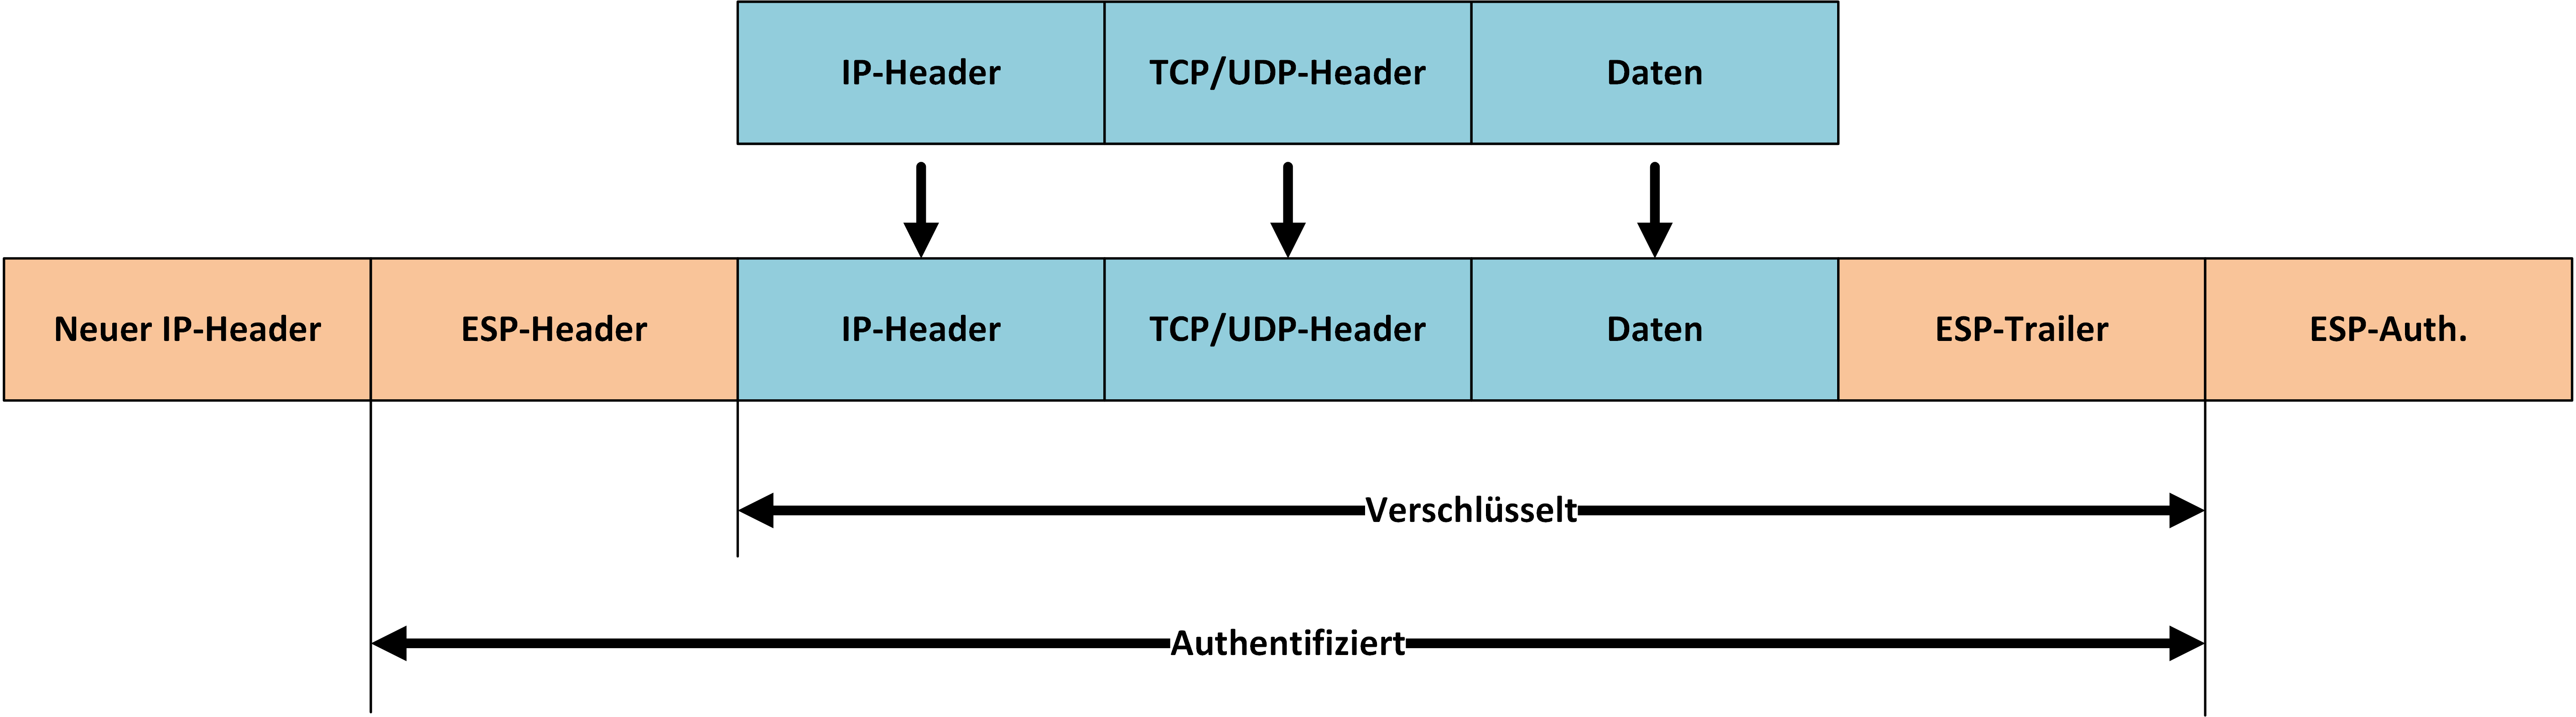
\includegraphics[trim=1 0 0 0,clip,width=\textwidth]{mainpart/analyse/img/ESP_Tunnelmode.png}
    \end{center}
    \caption{Aufbau eines Pakets im Tunnelmode}
\end{figure}

\noindent Bei einer Situation, in der nur zwei Rechner miteinander verbunden werden, kann der Transportmodus verwendet werden. Dieser Modus unterstützt nur Host-to-Host Verbindungen. Da es für \ac{IPsec} nicht unbedingt notwendig ist IP-Pakete vollständig neu zu entkapseln, können beim Transport Mode der originale IP-Header verwendet werden. Es kommen 8 Byte ESP-Header und 16-20Byte ESP-Trailer hinzu. Damit wird der Overhead kleiner, da man keinen zusätzlichen IP-Header benötigt.\cite{elektronik_kompendium}

\begin{figure}[H]
    \begin{center}
        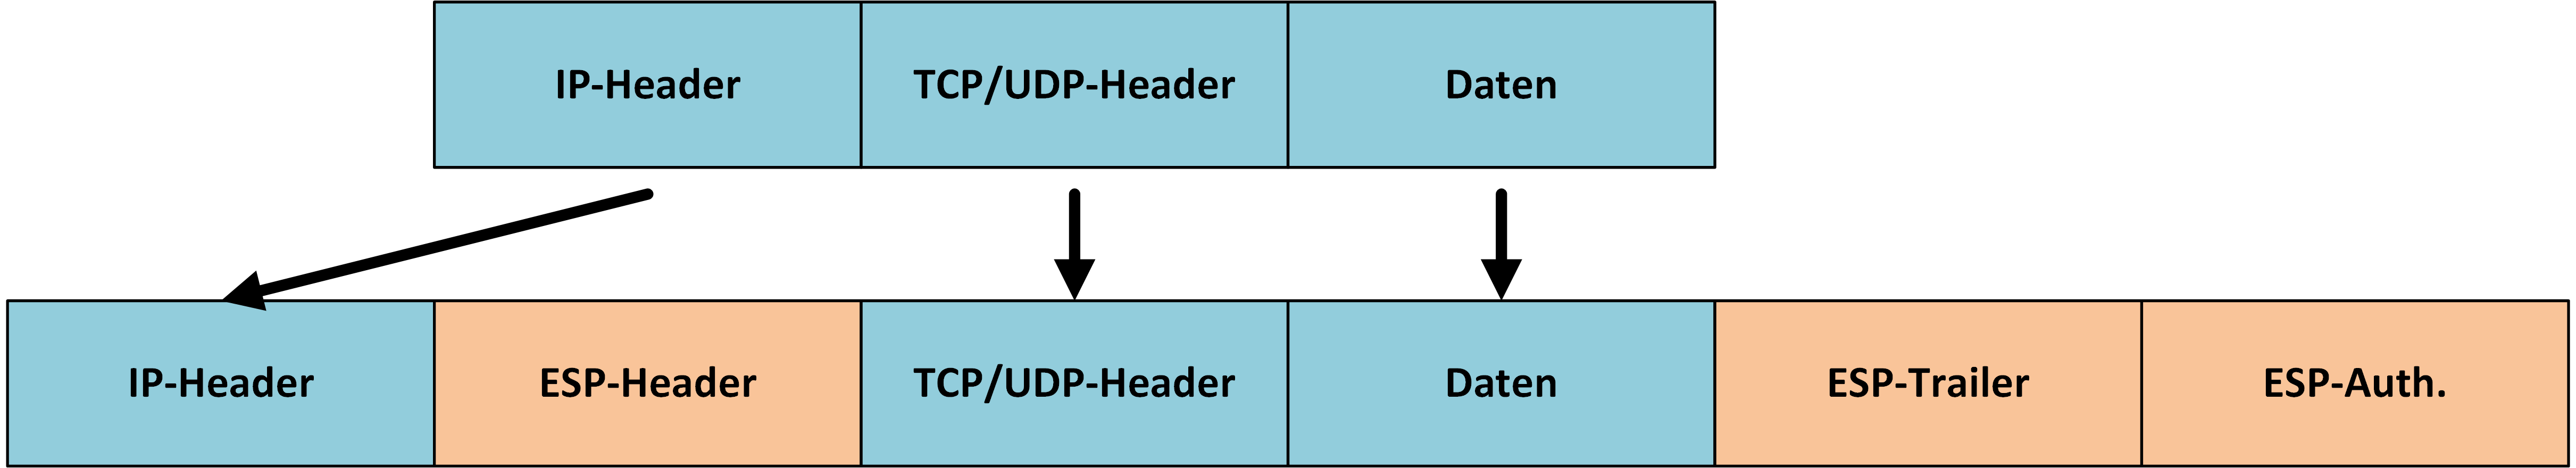
\includegraphics[trim=1 0 0 0,clip,width=\textwidth]{mainpart/analyse/img/ESP_Transportmode.png}
    \end{center}
    \caption{Aufbau eines Pakets im Transportmode}
    %\label{fig:AST_function_call_with_and_without_template_id}
\end{figure}


\textbf{Wichtige Felder}

\begin{table}[H]
\begin{tabularx}{\textwidth}{l|>{\raggedright\arraybackslash}X} 
\hline
Security Parameters\\ Index (SPI) 32bits & Dieser zufällig festgelegte Wert in Kombination mit der IP-Adresse des Ziels wird für eine Identifikation der Verbindung benötigt. Bei jeder neuen Verbindung wird die SPI neu gesetzt.                                                                                                                                                                                                                                                                         \\ \hline
Sequence Number 32bits & Die Sequence Number wird für jedes Paket gesetzt und wird danach für jedes neue Paket um 1 erhöht. Bei einer neuen Verbindung wird die Sequence Number stets auf 1 gesetzt. Falls Anti-Replay eingesetzt wird (standardmässig aktiviert) darf sich die Sequence Number nicht wiederholen. Daher wird, bevor das 2\^{}32 Paket gesendet wird, die Verbindung zurückgesetzt und eine neue SPI ausgehandelt. Damit ist auch die Sequence Number wieder zurückgesetzt. \\
\hline
\end{tabularx}
\caption{Wichtige ESP Felder}
\end{table}

\cleardoublepage
\section{MTU Discovery}

Netzwerk Pakete beinhalten typischerweise mehrere Netzwerkprotokolle. Diese Protokolle sind in Layern angeordnet und haben klar definierte Schnittstellen. Dadurch sind sie grösstenteils unabhängig voneinander und können ausgetauscht werden. Bei der Kommunikation mit einem Webserver hat man zum Beispiel den folgenden Aufbau\footnotemark[1]. HTTP über TCP/IP über Ethernet.

\begin{figure}[H]
    \begin{center}
        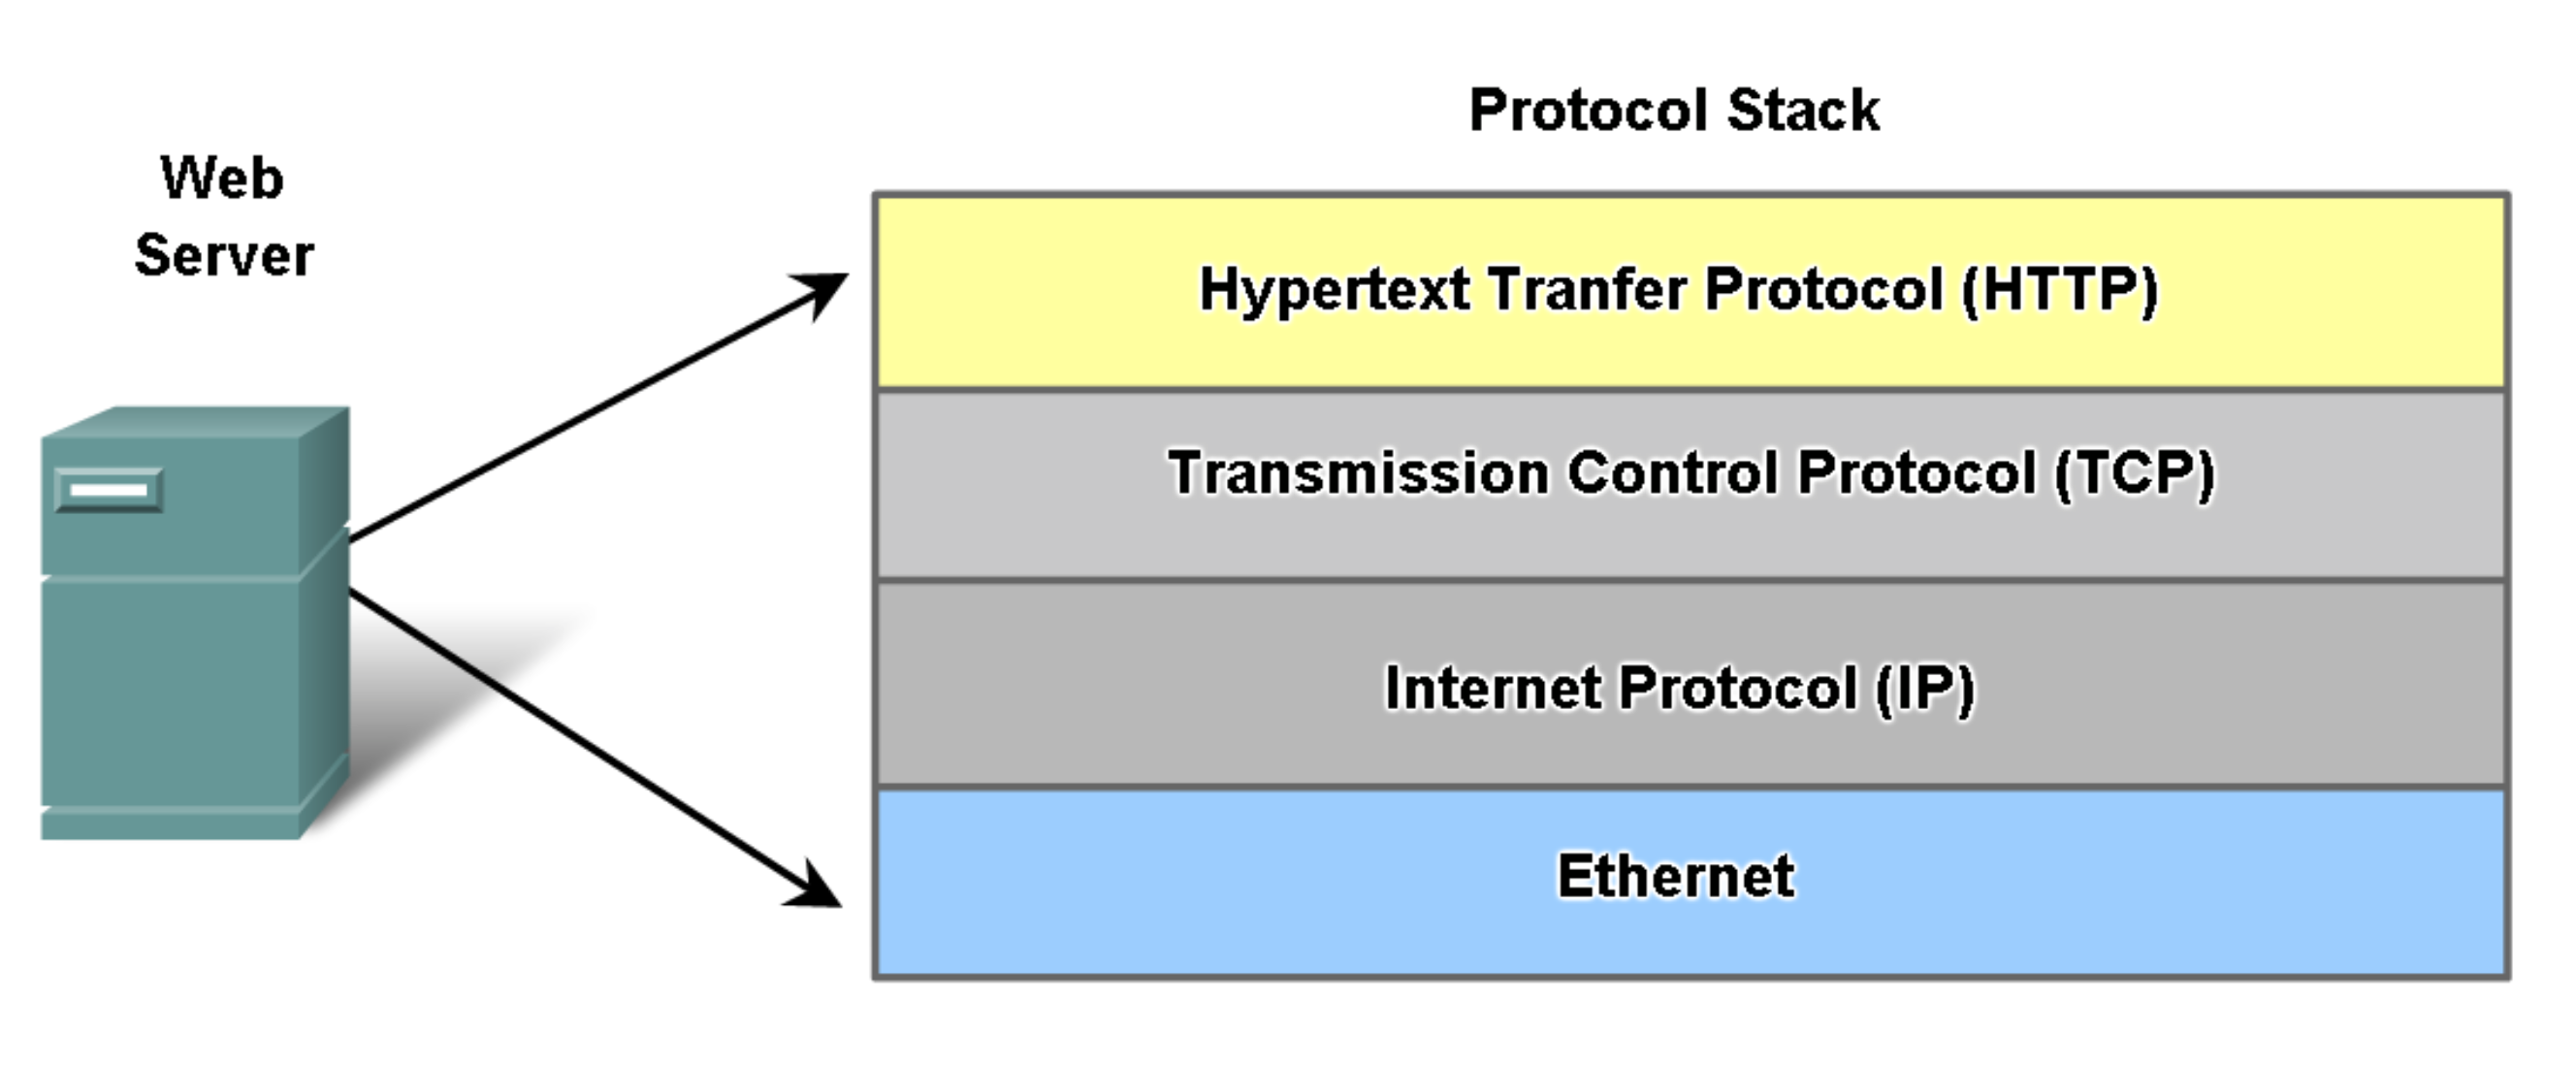
\includegraphics[trim=1 0 0 0,clip,width=\textwidth]{mainpart/analyse/img/HTTP_Stack}
    \end{center}
    \caption{Protokoll Stack eines typischen HTTP Requests}
\end{figure}

\footnotetext[1]{Bild: HSR Vorlesung CN1 - Steffen/Stettler, 29.07.2014, 1-Grundlagen.ppt}

Man ist aber nicht an genau diese Struktur gebunden. Man könnte zum Beispiel den Ethernet Layer durch einen anderen Layer austauschen und die restlichen Protokolle so belassen.

Um das Zusammenspiel der unterschiedlichen Netzwerk Layern besser zu veranschaulichen wurde das \ac{OSI}-Modell entwickelt. Das OSI Modell besteht aus 7 Layern die jeweils unterschiedliche Aufgaben haben. Protokolle die im gleichen \ac{OSI}-Layer mit klaren Schnittstellen definiert wurde sind einfach austauschbar.

\begin{figure}[H]
    \begin{center}
        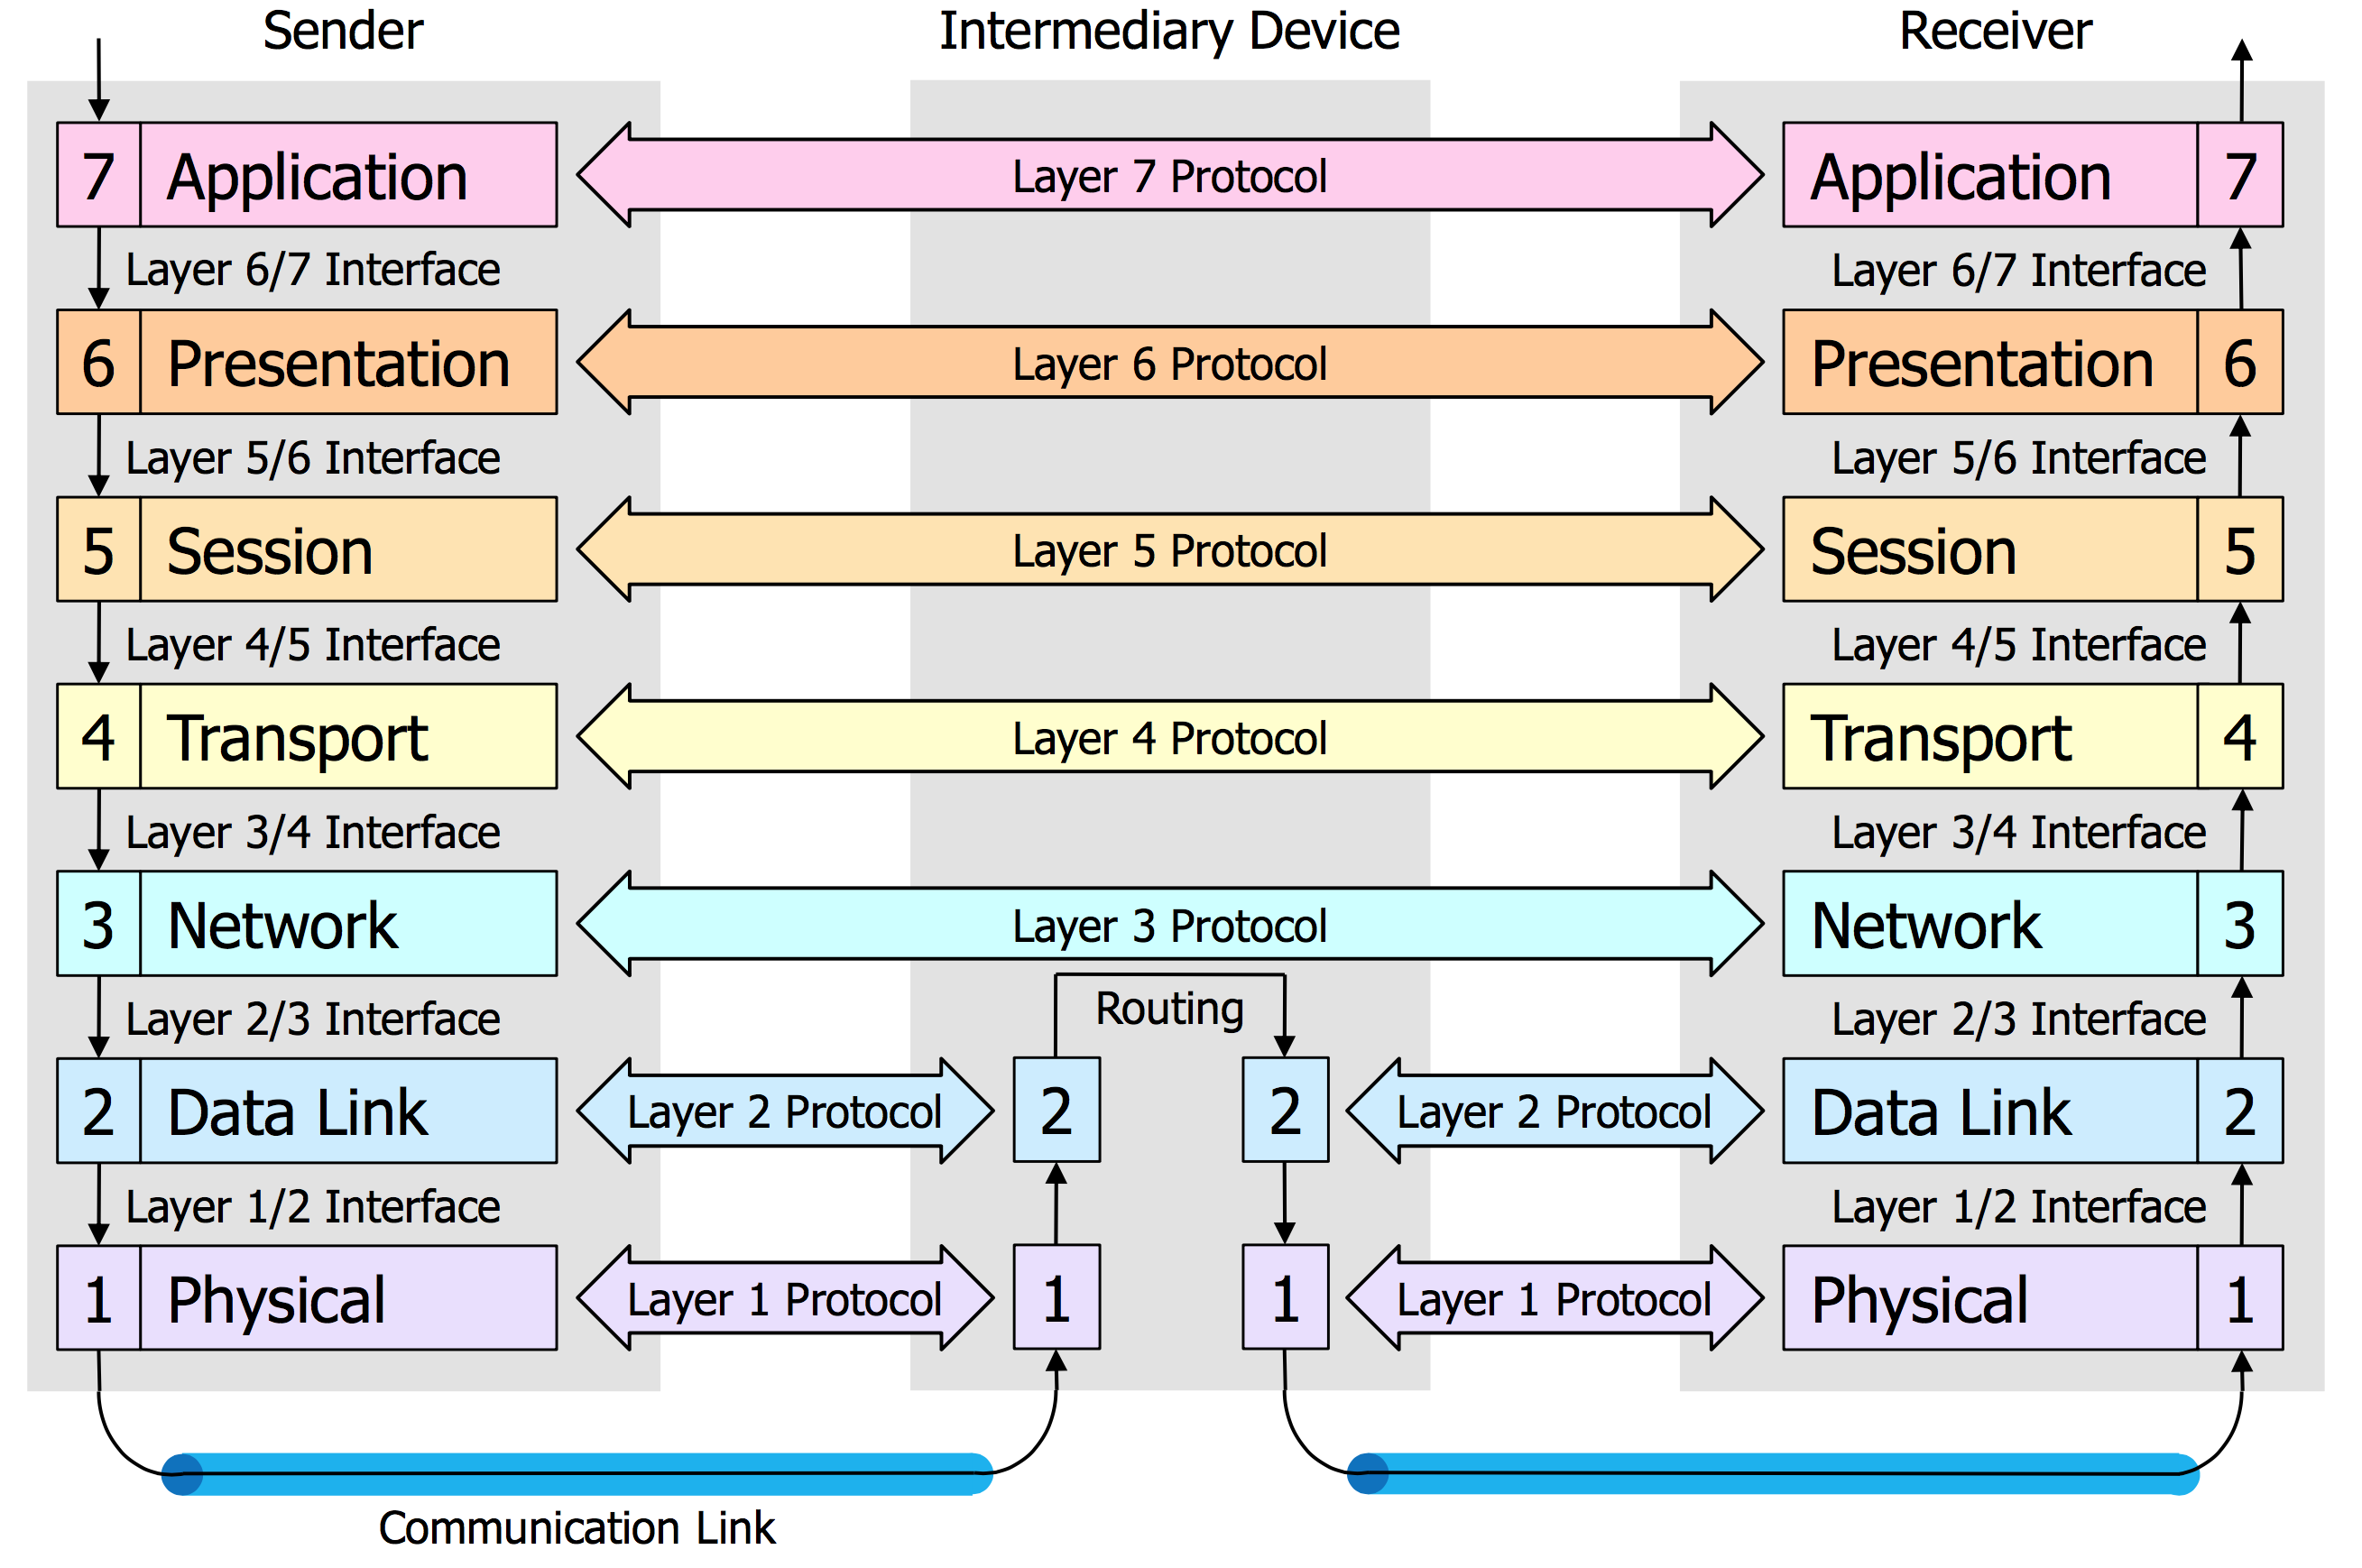
\includegraphics[trim=1 0 0 0,clip,width=\textwidth]{mainpart/analyse/img/OSI_Modell}
    \end{center}
    \caption{\ac{OSI} Referenzmodell}
\end{figure}

Für die \ac{MTU} Discovery sind vor allem die Layer 1,2,3 des \ac{OSI}-Modells\footnotemark[1] wichtig. In Layer 1 \& 2 findet die eigentliche physische Übertragung statt. So ist beispielsweise das Ethernet Protokoll sowohl im physischen Layer als auch im Data-Link-Layer vorhanden.

Die Protokolle der ersten beiden Layern haben im Vergleich zu den höheren Layern einen grossen Unterschied. Sie können nur eine begrenzt grosse Payload enthalten. So ist die maximale Payload bei Ethernet zum Beispiel 1500 Bytes. Ein Paket des Netzwerk-Layers (Layer 3) darf als maximal 1500 Bytes gross sein wenn es über Ethernet übertragen werden soll. Diese maximale Payload nennt man \acl{MTU} \acs{MTU}.

\footnotetext[1]{Bild: HSR Vorlesung CN1 - Steffen/Stettler, 29.07.2014, 1-Grundlagen.ppt}

Wenn ein Layer 3 Paket grösser als die \ac{MTU} ist dann muss es in mehrere Pakete aufgeteilt werden. Dieser Vorgang wird Fragmentierung genannt. Auch wenn Paket-Fragmentierung auftritt funktioniert eine Netzwerkverbindung normalerweise immer noch problemlos, es gibt jedoch auf Grund der Fragmentierung Performance-Einbussen. Daher versucht man, wenn möglich, Paket-Fragmentierung zu vermeiden.

\subsection{Hardware Abhängigkeit}
Die \ac{MTU} ist ein Hardware abhängiger Wert, der je nach der eingesetzten Technologie anders ist. Die Tabelle unten zeigt die \ac{MTU}s von einigen heute verwendeten Übertragungstechnologien.

\begin{table}[H]
\begin{tabularx}{\textwidth}{l|>{\raggedright\arraybackslash}X} 
\textbf{Technologie} & \textbf{MTU in Bytes} \\
\hline
\ac{FDDI} \cite[:915]{rfc1191} & 4352 \\
Ethernet \cite[:915]{rfc1191} & 1500 \\
\ac{PPPoE} \cite[:374]{rfc2516}& 1492 \\
X.25 Networks / ISDN \cite[:915]{rfc1191} & 576 \\
\end{tabularx}
\caption{Typische MTU-Grössen}
\end{table}

Wenn eine Verbindung von A nach B in mehrere Wegstrecken aufgeteilt ist und für diese Wegstrecken unterschiedliche Technologien verwendet werden dann ist die tiefste \ac{MTU} relevant für das Versenden von Paketen.

\subsection{Path MTU Discovery}
Da die \ac{MTU} bei einer neuen Verbindung noch unbekannt ist muss sie zuerst ermittelt werden. Normalerweise geschieht dies automatisch via \ac{PMTUD}. Dabei werden \ac{ICMP} Pakete unterschiedlicher Grösse die mit einem \enquote{Don't fragment} Flag versehen sind über die Verbindung gesandt. Wenn ein solches Paket auf ein Netzwerkgerät trifft dass nur eine tiefere \ac{MTU} unterstützt wird das Paket nicht weitergesendet, stattdessen wird ein \ac{ICMP} Paket mit dem Inhalt "Fragmentation needed" retourniert. So weiss der \ac{PMTUD} Algorithmus dass die \ac{MTU} der Verbindung überschritten wurde \cite[:131]{rfc1191}.

\ac{PMTUD} hat jedoch ein Problem. Router die, die \ac{ICMP} Pakete weiterleiten oder aber ein \enquote{Fragmentation needed} Paket zurücksenden sollten tun dies nicht immer. Dieses Fehlverhalten gibt es aus mehreren Gründen. Zum einen wegen Kernel-Bugs, Fehlkonfigurationen und zum anderen auch weil Firewalls manchmal so konfiguriert werden dass sie \ac{ICMP} Nachrichten nicht durchlassen auf Grund von Sicherheitsbedenken \cite[:137]{rfc2923}.

Da man sich also nicht auf \ac{PMTUD} verlassen kann um die \ac{MTU} einer Verbindung festzustellen wird mit dieser Arbeit eine \ac{MTU} Discovery implementiert die innerhalb einer \ac{IPsec} \ac{VPN} Verbindung durchgeführt werden kann.
